\begin{frame}
\frametitle{Efficient Algorithm?}
\vskip 1.0cm
    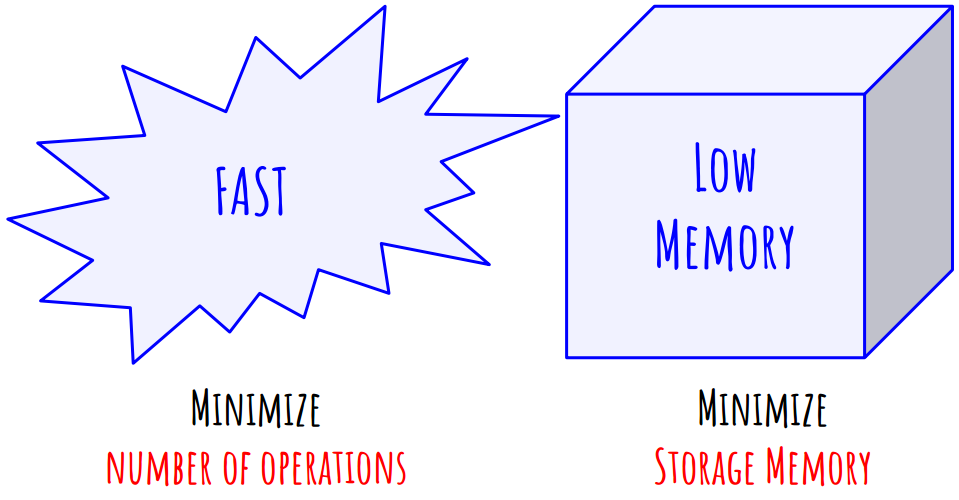
\includegraphics[width=1.0\textwidth]{./pictures/efficient.png}
\end{frame}

\begin{frame}
\frametitle{An example: simple average}
\vskip 0.6cm
\visible<2->{When measuring the average over \textcolor{isvblue}{2 reviews}:}
\begin{center}
    \visible<3->{$Average = \displaystyle{\frac{R_{1} + R_{2}}{2}}$} \qquad \visible<4->{\textcolor{isvblue}{$\rightarrow$ 2 operations}}
\end{center}

\visible<5->{When measuring the average over \textcolor{isvblue}{5 reviews}:}
\begin{center}
    \visible<6->{$Average = \displaystyle{\frac{R_{1} + R_{2} + R_3 + R_4 + R_5}{5}}$} \qquad \visible<7->{\textcolor{isvblue}{$\rightarrow$ 5 operations}}
\end{center}

\vskip 0.3cm
\visible<8->{\textbf{When measuring the average over \textcolor{isvblue}{N reviews}:}}
\begin{center}
    \visible<9->{$Average = \displaystyle{\frac{R_{1} + R_{2} + ...  + R_N}{N}}$} \qquad \visible<10->{\textcolor{isvblue}{\textbf{$\rightarrow$ N operations}}}
\end{center}
\visible<11->{\textbf{Storage memory:}} \visible<12->{\textcolor{isvblue}{\textbf{1 single value (decimal), the Average}}}
\end{frame}
